\documentclass[a4paper,14pt]{article}
\usepackage{extsizes}
\usepackage[utf8]{inputenc}
\usepackage[T1]{fontenc}
\usepackage[bulgarian]{babel}
\usepackage{amsmath}
\usepackage [full]{textcomp}
\usepackage{graphicx}
\DeclareGraphicsExtensions{.pdf,.png,.jpg}
\usepackage[hmargin=3cm,vmargin=2cm]{geometry}
\usepackage{hyperref}


\title{
\vspace{2.0cm}
\begin{large}
Курсов проект по \\
Системи за електронен бизнес
\end{large}
\vspace{2.5cm}
\hline
\vspace{0.5cm}
\textbf{Електронна търговия
\\ \vspace{0.5cm} с картини}
\vspace{0.5cm}
\hline
\\ \vspace{2.5cm}
\\ \vspace{0.5cm}\Large{\textit{Преподавател:} \\ доц. д-р Павел Павлов}
\\ \vspace{1.0cm}\Large{\textit{Автор:} \\ Валентина Динкова, ф.н. 71112, 2 група}}

\begin{document}
\maketitle

\newpage

\tableofcontents

\newpage
\section{Увод}
Проектът създава онлайн магазин за електронна търговия с картини. Обслужва два типа потребители - администратор и клиент. Администраторите отговарят
за поддържането и контрола на данните: добавят нови картини, редактират съществуващи такива. Преглеждат заявки за закупуване на картини
и извършват продажбата им. Клиентът разглежда каталог със картини. Има възможност за
търсене по различни критерии. Има възможност да добави в потребителската количка една или повече картини и да ги закупи. Може да види сумата, която трябва да заплати, да прибавя, изважда картини от своята потребителска количка.


\section{Архитектура}


\subsection{Използвани среди и технологии}
За изготвянето на проекта са използвани ASP.NET и C\#. Методите, използвани за изготвянето на проекта са по образец от примера,
 показан в книгата \textit{“Beginning ASP.NET E-Commerce in C\# 2005: From Novice to Professional”} на издателство \textit{Apress}.
 
 За целта съм използвала следния софтуер:
 \begin{itemize}
\item
Microsoft Visual Studio 2010
\item
Microsoft SQL Server 2008 R2
\item
SQL Server Management Studio Express
\end{itemize}

Използванa е трислойна архитектура (3-tier architecture):
\begin{enumerate}
\item
\textbf{Презентационен слой (presentation tier)} – предоставя потребителския интерфейс; реализиран е на ASP.NET
\item
\textbf{Бизнес слой (business tier)} – слой посредник между другите два, реализира логиката на приложението. Той се програмира на езика C\#
\item
\textbf{Слой за съхранение и обработка на базата данни (data tier)} -  С помощтта на Stored Procedures бизнес слоя си комуникира с базата от данни.
\end{enumerate}
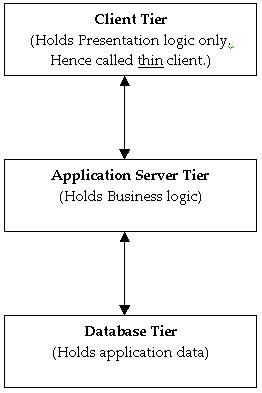
\includegraphics{21}



\subsection{Етапи на разработка}

Проектът за електронна галерия е изграден на няколко етапа:
\begin{enumerate}
\item
\textbf{Първи етап} - реализирани са категориите и подкатегориите на стоките, описанията на стоките, търсенето в каталога, отделите.
\item
\textbf{Втори етап} - реализирани са потребителската кошница, която съхранява данните за продуктите, добавени в нея в базата данни за всеки клиент, като има възможност за редактиране на съдържанието и обработка на поръчките. Освен това се реализира и система за препоръки на стоки от магазина.

\item
\textbf{Трети етап} - реализира се частта за потребителските сметки, обработване на потребителските поръчки, проверка за наличност в склад.
\end{enumerate}

\subsection{База от данни}
За проекта е използвана системата за управление на бази от данни Microsoft SQL Server
2008 R2 Express. На този етап са създадени всички таблици в базата от данни, поддържащи
системата, както и връзките между тях, различни ограничения и някои съхранени процедури
(stored procedures).
\\
\\
\textbf{Product} Съдържа информация за продуктите, налични в базата от данни. Пази се информация за:
\begin{itemize}
\item име, описание, цена на картината;
\item автор на картината;
\item използвана техника;
\item снимка - линк към снимка на картината;
\item дата;
\end{itemize}
\\
\textbf{Orders} Съдържа информация за поръчките, налични в базата от данни. Пази се информация за:
\begin{itemize}
\item дата на поръчката;
\item дата на доставката;
\item флаг: верифицирана;
\item флаг: завършена;
\item флаг: отменена;
\item коментари;
\item име на клиента;
\item email на клиента;
\item адрес за доставка;
\item идентификатор на клиента;
\item идентификатор на авторизацията.
\end{itemize}
\\
\textbf{OrderDetails} Данни относно поръчка. Пази се информация за:
\begin{itemize}
\item номер на поръчката;
\item количество;
\item единична цена;
\item подсума (количество * цена).
\end{itemize}
\\
\textbf{Tax} Съдържа информация за данъците, отнасящи се към дадено множество от поръчки.\\
\textbf{ShippingRegion} Регион на доставка.\\
\textbf{Shipping} Доставка:
\begin{itemize}
\item цена;
\item връзка към региона за доставка;
\item тип на доставката.
\end{itemize}
\\
\textbf{Audit} Таблица, съдържаща информация за одити на поръчките. \\
\textbf{ProductAttributeValue} Съдържа информация за различни атрибути на картините, извън по-
летата на \textbf{Product}. Тази таблица е свързваща за таблиците \textbf{Product} и \textbf{AttributeValue}.\\
\textbf{AttributeValue} свързва име на даден атрибут с конкретната му стойност.\\
\textbf{ShoppingCart} Представлява артикул в количката на клиента. Всеки клиент има уникална
количка, отличаваща се с \textit{CartID} идентификатор.

\end{document}